\documentclass[12pt]{article}
\usepackage[utf8]{inputenc}
\usepackage{amsmath}
\usepackage{amssymb}
\usepackage{geometry}
\usepackage{pgfplots}
\usepackage{tikz}
\geometry{margin=1in}
\pgfplotsset{compat=1.17}

\title{Campos Vectoriales y Procedimientos de Ecuaciones Diferenciales}
\author{}
\date{}

\begin{document}
\maketitle

\section*{Campos Vectoriales}

\subsection*{1.- Campo vectorial del Ejercicio 1}
\begin{minipage}[t]{0.5\textwidth}
\textbf{Procedimiento:}
\[
2y\,dy - (2y - 10x)\,dx = 0
\]
\[
2y\,dy = (2y - 10x)dx
\]
\[
\int 2y\,dy = \int (2y - 10x)dx
\]
\[
y^2 = 2xy - 5x^2 + C
\]
\end{minipage}
\hfill
\begin{minipage}[t]{0.45\textwidth}
\begin{center}
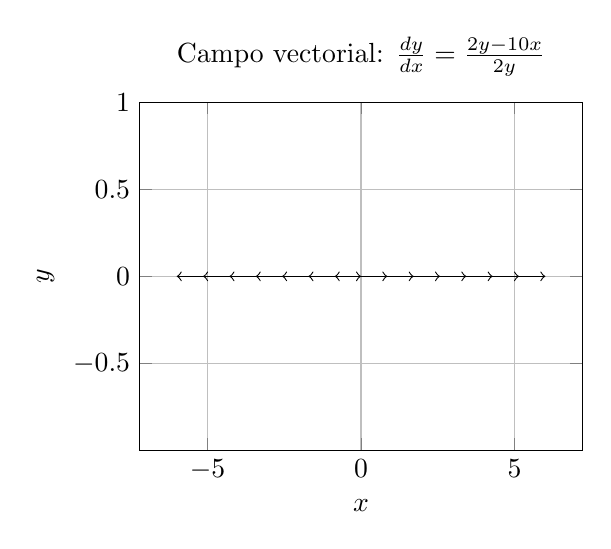
\begin{tikzpicture}
\begin{axis}[
    width=7.2cm,
    height=6cm,
    xlabel={$x$},
    ylabel={$y$},
    title={Campo vectorial: $\frac{dy}{dx}=\frac{2y-10x}{2y}$},
    grid=major,
    domain=-3:3,
    range=-3:3,
]
\addplot[quiver={u={2*y-10*x},v={2*y},scale arrows=0.3},->,samples=15] {0};
\end{axis}
\end{tikzpicture}
\end{center}
\end{minipage}

\vspace{1cm}

\subsection*{2.- Campo vectorial del Ejercicio 2}
\begin{minipage}[t]{0.5\textwidth}
\textbf{Procedimiento:}
\[
y' = 3x^2
\]
\[
\frac{dy}{dx} = 3x^2
\]
\[
dy = 3x^2dx
\]
\[
\int dy = \int 3x^2dx
\]
\[
y = x^3 + C
\]
\end{minipage}
\hfill
\begin{minipage}[t]{0.45\textwidth}
\begin{center}
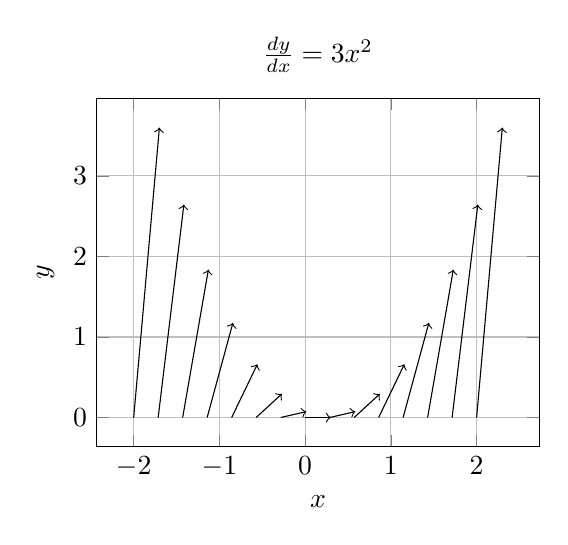
\begin{tikzpicture}
\begin{axis}[
    width=7.2cm,
    height=6cm,
    xlabel={$x$},
    ylabel={$y$},
    title={$\frac{dy}{dx}=3x^2$},
    grid=major,
    domain=-2:2,
    range=-2:2,
]
\addplot[quiver={u={1},v={3*x^2},scale arrows=0.3},->,samples=15] {0};
\end{axis}
\end{tikzpicture}
\end{center}
\end{minipage}

\vspace{1cm}

\subsection*{3.- Campo vectorial del Ejercicio 3}
\begin{minipage}[t]{0.5\textwidth}
\textbf{Procedimiento:}
\[
y' = x + 1
\]
\[
\frac{dy}{dx}=x+1
\]
\[
dy=(x+1)dx
\]
\[
\int dy = \int (x+1)dx
\]
\[
y = \frac{x^2}{2}+x+C
\]
\end{minipage}
\hfill
\begin{minipage}[t]{0.45\textwidth}
\begin{center}
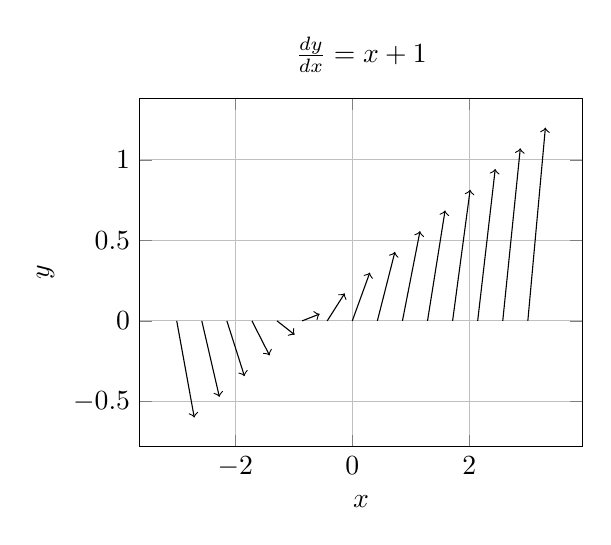
\begin{tikzpicture}
\begin{axis}[
    width=7.2cm,
    height=6cm,
    xlabel={$x$},
    ylabel={$y$},
    title={$\frac{dy}{dx}=x+1$},
    grid=major,
    domain=-3:3,
    range=-3:3,
]
\addplot[quiver={u={1},v={x+1},scale arrows=0.3},->,samples=15] {0};
\end{axis}
\end{tikzpicture}
\end{center}
\end{minipage}

\vspace{1cm}

\subsection*{4.- Campo vectorial del Ejercicio 4}
\begin{minipage}[t]{0.5\textwidth}
\textbf{Procedimiento:}
\[
\frac{dy}{y}=5\,dt
\]
\[
\int \frac{dy}{y}=\int 5dt
\]
\[
\ln|y|=5t+C
\]
\[
|y|=Ce^{5t}
\]
\end{minipage}
\hfill
\begin{minipage}[t]{0.45\textwidth}
\begin{center}
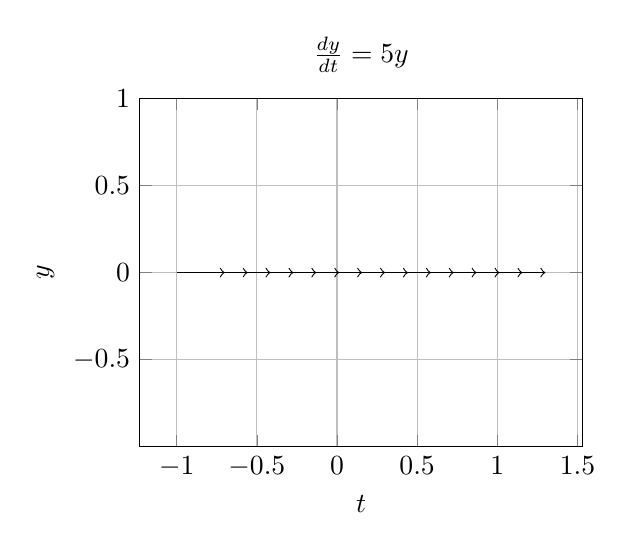
\begin{tikzpicture}
\begin{axis}[
    width=7.2cm,
    height=6cm,
    xlabel={$t$},
    ylabel={$y$},
    title={$\frac{dy}{dt}=5y$},
    grid=major,
    domain=-1:1,
    range=-3:3,
]
\addplot[quiver={u={1},v={5*y},scale arrows=0.3},->,samples=15] {0};
\end{axis}
\end{tikzpicture}
\end{center}
\end{minipage}

\vspace{1cm}

\subsection*{5.- Campo vectorial del Ejercicio 5}
\begin{minipage}[t]{0.5\textwidth}
\textbf{Procedimiento:}
\[
(8x+1)dx+2y\,dy=0
\]
\[
2y\,dy=-(8x+1)dx
\]
\[
\int 2y\,dy=-\int(8x+1)dx
\]
\[
y^2=-4x^2-x+C
\]
\end{minipage}
\hfill
\begin{minipage}[t]{0.45\textwidth}
\begin{center}
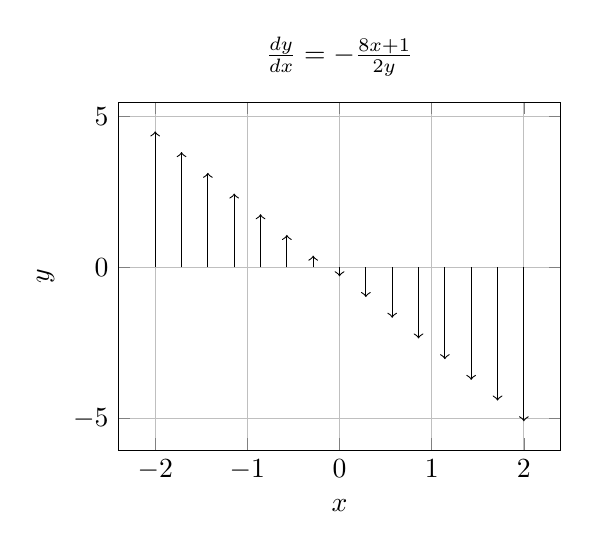
\begin{tikzpicture}
\begin{axis}[
    width=7.2cm,
    height=6cm,
    xlabel={$x$},
    ylabel={$y$},
    title={$\frac{dy}{dx}=-\frac{8x+1}{2y}$},
    grid=major,
    domain=-2:2,
    range=-3:3,
]
\addplot[quiver={u={2*y},v={-(8*x+1)},scale arrows=0.3},->,samples=15] {0};
\end{axis}
\end{tikzpicture}
\end{center}
\end{minipage}

\vspace{1cm}

\subsection*{6.- Campo vectorial del Ejercicio 6}
\begin{minipage}[t]{0.5\textwidth}
\textbf{Procedimiento:}
\[
y^2dy=(x+2)dx
\]
\[
\int y^2dy=\int(x+2)dx
\]
\[
\frac{y^3}{3}=\frac{x^2}{2}+2x+C
\]
\[
y^3=\frac{3x^2}{2}+6x+C
\]
\end{minipage}
\hfill
\begin{minipage}[t]{0.45\textwidth}
\begin{center}
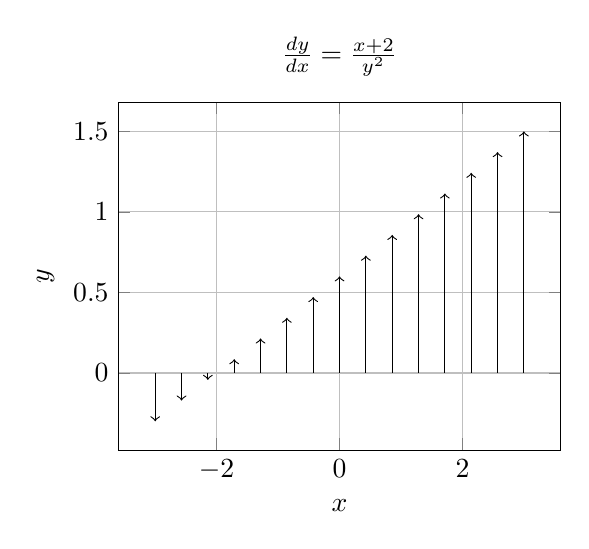
\begin{tikzpicture}
\begin{axis}[
    width=7.2cm,
    height=6cm,
    xlabel={$x$},
    ylabel={$y$},
    title={$\frac{dy}{dx}=\frac{x+2}{y^2}$},
    grid=major,
    domain=-3:3,
    range=-3:3,
]
\addplot[quiver={u={y^2},v={x+2},scale arrows=0.3},->,samples=15] {0};
\end{axis}
\end{tikzpicture}
\end{center}
\end{minipage}

\vspace{1cm}

\subsection*{7.- Campo vectorial del Ejercicio 7}
\begin{minipage}[t]{0.5\textwidth}
\textbf{Procedimiento:}
\[
(6y-\sec^2y)dy-(1+\sin x)dx=0
\]
\[
(6y-\sec^2y)dy=(1+\sin x)dx
\]
\[
\int(6y-\sec^2y)dy=\int(1+\sin x)dx
\]
\[
3y^2-\tan y=x-\cos x+C
\]
\end{minipage}
\hfill
\begin{minipage}[t]{0.45\textwidth}
\begin{center}
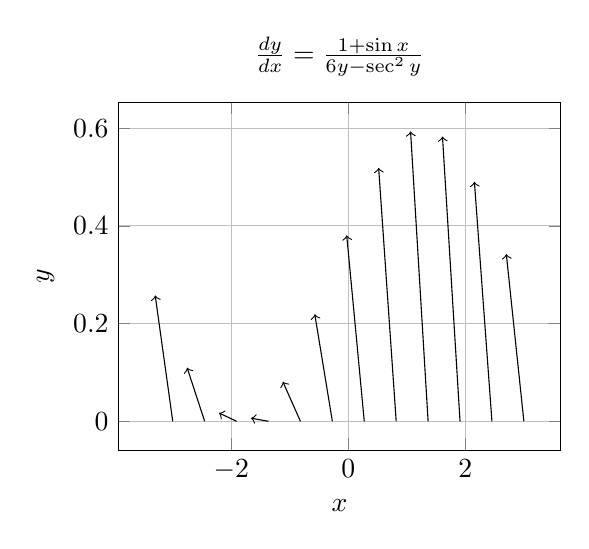
\begin{tikzpicture}
\begin{axis}[
    width=7.2cm,
    height=6cm,
    xlabel={$x$},
    ylabel={$y$},
    title={$\frac{dy}{dx}=\frac{1+\sin x}{6y-\sec^2y}$},
    grid=major,
    domain=-3:3,
    range=-1.5:1.5,
]
\addplot[quiver={u={6*y-1/cos(deg(y))^2},v={1+sin(deg(x))},scale arrows=0.3},->,samples=12] {0};
\end{axis}
\end{tikzpicture}
\end{center}
\end{minipage}

\vspace{1cm}

\subsection*{8.- Campo vectorial del Ejercicio 8}
\begin{minipage}[t]{0.5\textwidth}
\textbf{Procedimiento:}
\[
\frac{e^y y'}{6}=e^{2x}
\]
\[
e^y\,dy=6e^{2x}dx
\]
\[
\int e^y dy = \int 6e^{2x}dx
\]
\[
e^y=3e^{2x}+C
\]
\[
y=\ln(3e^{2x}+C)
\]
\end{minipage}
\hfill
\begin{minipage}[t]{0.45\textwidth}
\begin{center}
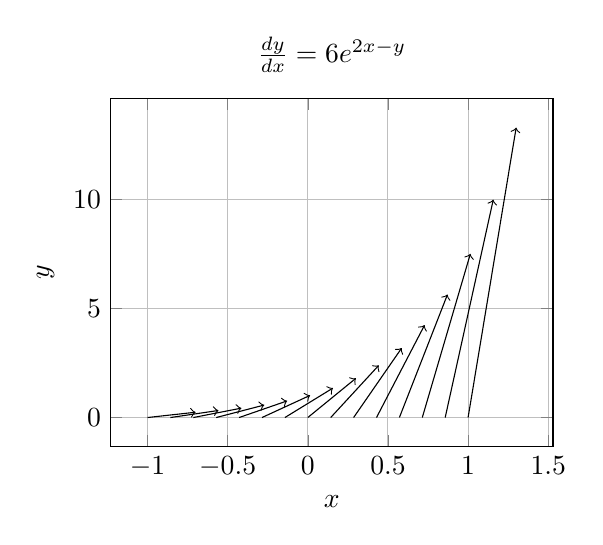
\begin{tikzpicture}
\begin{axis}[
    width=7.2cm,
    height=6cm,
    xlabel={$x$},
    ylabel={$y$},
    title={$\frac{dy}{dx}=6e^{2x-y}$},
    grid=major,
    domain=-1:1,
    range=-2:2,
]
\addplot[quiver={u={1},v={6*exp(2*x-y)},scale arrows=0.3},->,samples=15] {0};
\end{axis}
\end{tikzpicture}
\end{center}
\end{minipage}

\vspace{1cm}

\subsection*{9.- Campo vectorial del Ejercicio 9}
\begin{minipage}[t]{0.5\textwidth}
\textbf{Procedimiento:}
\[
x' = \frac{x^2y^2}{1+x}
\]
\[
\frac{dx}{dy}=\frac{x^2y^2}{1+x}
\]
\[
\frac{1+x}{x^2}dx=y^2dy
\]
\[
\left(\frac{1}{x^2}+\frac{1}{x}\right)dx=y^2dy
\]
\[
-\frac{1}{x}+\ln|x|=\frac{y^3}{3}+C
\]
\end{minipage}
\hfill
\begin{minipage}[t]{0.45\textwidth}
\begin{center}
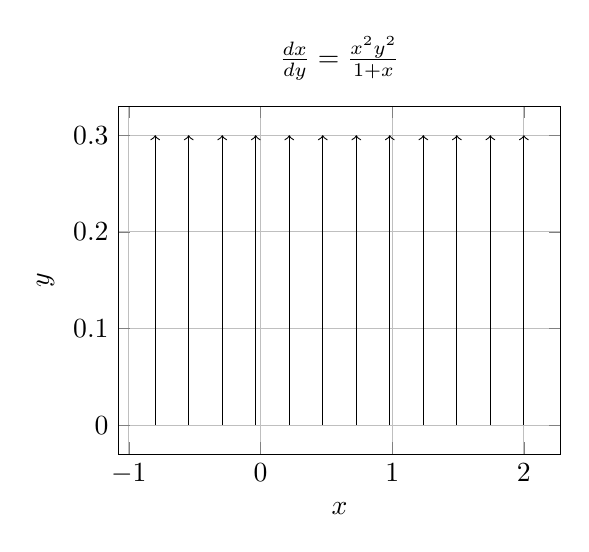
\begin{tikzpicture}
\begin{axis}[
    width=7.2cm,
    height=6cm,
    xlabel={$x$},
    ylabel={$y$},
    title={$\frac{dx}{dy}=\frac{x^2y^2}{1+x}$},
    grid=major,
    domain=-0.8:2,
    range=-2:2,
]
\addplot[quiver={u={x^2*y^2/(1+x)},v={1},scale arrows=0.3},->,samples=12] {0};
\end{axis}
\end{tikzpicture}
\end{center}
\end{minipage}

\vspace{1cm}

\subsection*{10.- Campo vectorial del Ejercicio 10}
\begin{minipage}[t]{0.5\textwidth}
\textbf{Procedimiento:}
\[
y' = \frac{1+2x^2}{x\sin y}
\]
\[
\sin y\,dy = \frac{1+2x^2}{x}dx
\]
\[
\sin y\,dy = \left(\frac{1}{x}+2x\right)dx
\]
\[
-\cos y = \ln|x|+x^2+C
\]
\[
\cos y = -\ln|x|-x^2+C
\]
\end{minipage}
\hfill
\begin{minipage}[t]{0.45\textwidth}
\begin{center}
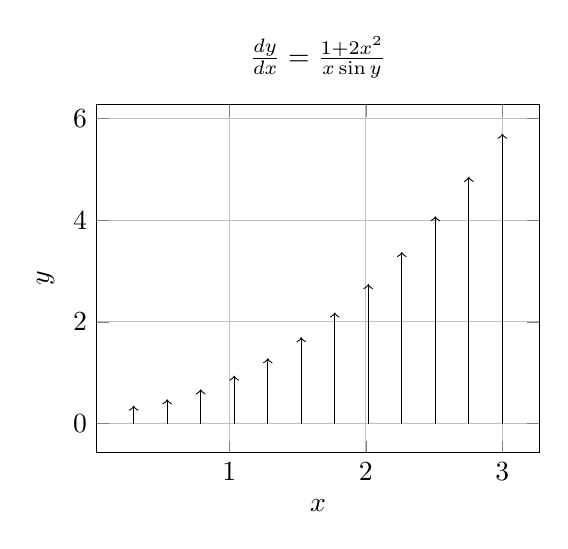
\begin{tikzpicture}
\begin{axis}[
    width=7.2cm,
    height=6cm,
    xlabel={$x$},
    ylabel={$y$},
    title={$\frac{dy}{dx}=\frac{1+2x^2}{x\sin y}$},
    grid=major,
    domain=0.3:3,
    range=0.3:3,
]
\addplot[quiver={u={x*sin(deg(y))},v={1+2*x^2},scale arrows=0.3},->,samples=12] {0};
\end{axis}
\end{tikzpicture}
\end{center}
\end{minipage}

\vspace{1cm}

\subsection*{11.- Campo vectorial del Ejercicio 11}
\begin{minipage}[t]{0.5\textwidth}
\textbf{Procedimiento:}
\[
(y^2+xy^2)dy=z^0dx
\]
Como $z^0=1$:
\[
y^2(1+x)dy=dx
\]
\[
y^2dy = \frac{dx}{1+x}
\]
\[
\int y^2dy = \int \frac{dx}{1+x}
\]
\[
\frac{y^3}{3}=\ln|1+x|+C
\]
\end{minipage}
\hfill
\begin{minipage}[t]{0.45\textwidth}
\begin{center}
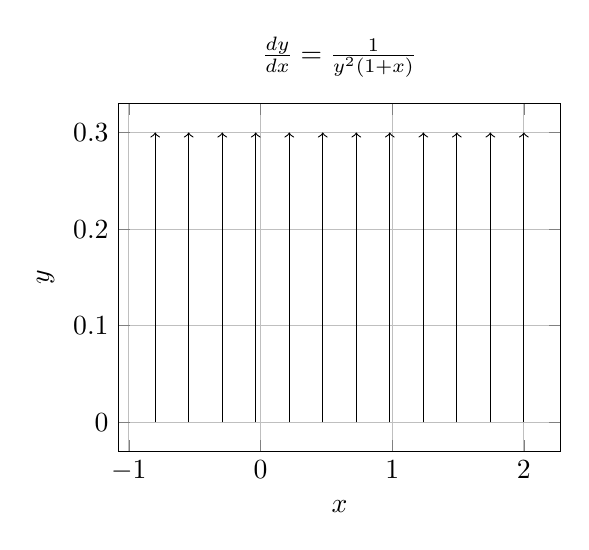
\begin{tikzpicture}
\begin{axis}[
    width=7.2cm,
    height=6cm,
    xlabel={$x$},
    ylabel={$y$},
    title={$\frac{dy}{dx}=\frac{1}{y^2(1+x)}$},
    grid=major,
    domain=-0.8:2,
    range=-2:2,
]
\addplot[quiver={u={y^2*(1+x)},v={1},scale arrows=0.3},->,samples=12] {0};
\end{axis}
\end{tikzpicture}
\end{center}
\end{minipage}

\vspace{1cm}

\subsection*{12.- Campo vectorial del Ejercicio 12}
\begin{minipage}[t]{0.5\textwidth}
\textbf{Procedimiento:}
\[
yy' = e^x-y^2
\]
\[
y\frac{dy}{dx}=e^x-y^2
\]
\[
\int y\,dy = \int (e^x-y^2)dx
\]
\[
\text{Se resuelve por sustituci\'on}
\]
\end{minipage}
\hfill
\begin{minipage}[t]{0.45\textwidth}
\begin{center}
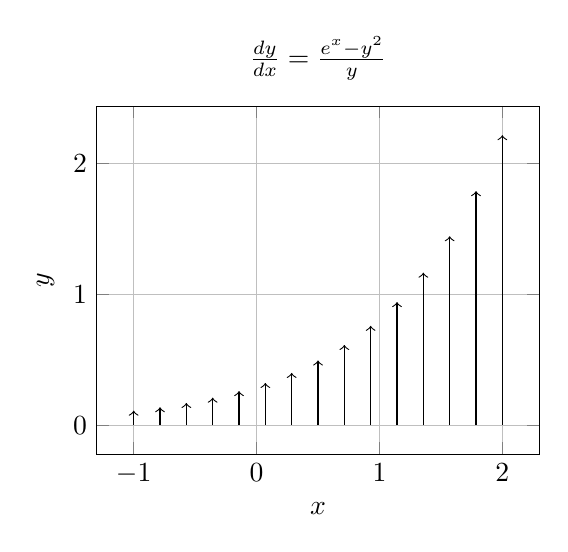
\begin{tikzpicture}
\begin{axis}[
    width=7.2cm,
    height=6cm,
    xlabel={$x$},
    ylabel={$y$},
    title={$\frac{dy}{dx}=\frac{e^x-y^2}{y}$},
    grid=major,
    domain=-1:2,
    range=-3:3,
]
\addplot[quiver={u={y},v={exp(x)-y^2},scale arrows=0.3},->,samples=15] {0};
\end{axis}
\end{tikzpicture}
\end{center}
\end{minipage}

\vspace{1cm}

\subsection*{13.- Campo vectorial del Ejercicio 13}
\begin{minipage}[t]{0.5\textwidth}
\textbf{Procedimiento:}
\[
e^x y' = e^{2x}+2y
\]
\[
\frac{dy}{dx}=e^x+2e^{-x}y
\]
\[
\frac{dy}{dx}-2e^{-x}y=e^x
\]
\[
\text{Ecuaci\'on lineal de primer orden}
\]
\end{minipage}
\hfill
\begin{minipage}[t]{0.45\textwidth}
\begin{center}
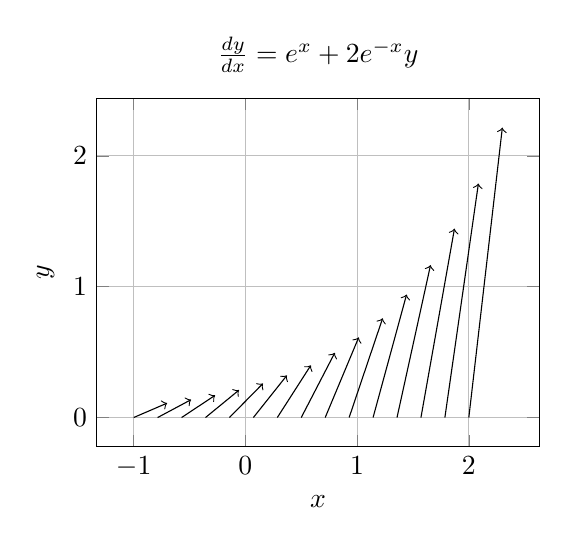
\begin{tikzpicture}
\begin{axis}[
    width=7.2cm,
    height=6cm,
    xlabel={$x$},
    ylabel={$y$},
    title={$\frac{dy}{dx}=e^x+2e^{-x}y$},
    grid=major,
    domain=-1:2,
    range=-2:2,
]
\addplot[quiver={u={1},v={exp(x)+2*exp(-x)*y},scale arrows=0.3},->,samples=15] {0};
\end{axis}
\end{tikzpicture}
\end{center}
\end{minipage}

\vspace{1cm}

\subsection*{14.- Campo vectorial del Ejercicio 14}
\begin{minipage}[t]{0.5\textwidth}
\textbf{Procedimiento:}
\[
y' = \frac{x^2}{y^3}
\]
\[
y^3dy=x^2dx
\]
\[
\int y^3dy = \int x^2dx
\]
\[
\frac{y^4}{4}=\frac{x^3}{3}+C
\]
\[
y^4=\frac{4}{3}x^3+C
\]
Usando $y(0)=1$:
\[
1 = \frac{4}{3}(0)^3 + C \Rightarrow C=1
\]
\[
y = \sqrt[4]{\frac{4}{3}x^3+1}
\]
\end{minipage}
\hfill
\begin{minipage}[t]{0.45\textwidth}
\begin{center}
\begin{tikzpicture}
\begin{axis}[
    width=7.2cm,
    height=6cm,
    xlabel={$x$},
    ylabel={$y$},
    title={$\frac{dy}{dx}=\frac{x^2}{y^3}$},
    grid=major,
    domain=-2:2,
    range=0.5:2.5,
]
\addplot[quiver={u={1},v={x^2/y^3},scale arrows=0.3},->,samples=15] {0};
\end{axis}
\end{tikzpicture}
\end{center}
\end{minipage}

\vspace{1cm}

\subsection*{15.- Campo vectorial del Ejercicio 15}
\begin{minipage}[t]{0.5\textwidth}
\textbf{Procedimiento:}
\[
y' + ty = y
\]
\[
y' + (t-1)y = 0
\]
\[
\frac{dy}{dt} = (1-t)y
\]
\[
\frac{dy}{y}=(1-t)dt
\]
\[
\int\frac{dy}{y}=\int(1-t)dt
\]
\[
\ln|y|=t-\frac{t^2}{2}+C
\]
\[
|y|=Ce^{t-\frac{t^2}{2}}
\]
Con $y(1)=3$:
\[
3=Ce^{1-\frac{1}{2}}=Ce^{1/2}
\]
\[
C=3e^{-1/2}
\]
\[
|y|=3e^{t-\frac{t^2}{2}-\frac12}
\]
\end{minipage}
\hfill
\begin{minipage}[t]{0.45\textwidth}
\begin{center}
\begin{tikzpicture}
\begin{axis}[
    width=7.2cm,
    height=6cm,
    xlabel={$t$},
    ylabel={$y$},
    title={$\frac{dy}{dt}=(1-t)y$},
    grid=major,
    domain=-1:3,
    range=-2:5,
]
\addplot[quiver={u={1},v={(1-t)*y},scale arrows=0.3},->,samples=15] {0};
\end{axis}
\end{tikzpicture}
\end{center}
\end{minipage}

\end{document}
